\documentclass[11pt]{article} % use larger type; default would be 10pt
\usepackage{amsmath}
\usepackage{tikz}
\usepackage{geometry} % to change the page dimensions
\geometry{a4paper} % or letterpaper (US) or a5paper or....
\geometry{margin=1in}
\usepackage{circuitikz}
\usepackage{float} % For the H position specifier

\usepackage{graphicx}
\usepackage{caption}
\usepackage{subcaption} % For subfigures
\usepackage{amsmath} % pretty maths
\usepackage{amsfonts}
\usepackage{amssymb}
\usepackage{fancyhdr} % This should be set AFTER setting up the page geometry
\pagestyle{fancy} % options: empty , plain , fancy
\renewcommand{\headrulewidth}{0pt} % customise the layout...
\lhead{ES3C5}\chead{}\rhead{Signal Processing}
\lfoot{}\cfoot{\thepage}\rfoot{}


\usepackage{amsthm}

\theoremstyle{definition}
\newtheorem{example}{Example}[subsection]

\begin{document}

\section{Signals}
	\begin{itemize}
	\item A quantity that can be varied to convey information
	\item Converted into electrical form using a transducer
	\item e.g. sine waves
		
	\end{itemize}

	\begin{figure}[h]
		\begin{tikzpicture}
			\draw (0,0) -- (1,0) -- (1,1) -- (2,1) --(2,0) -- (3,0);
		\end{tikzpicture}
		\centering
		\caption{A square wave for some reason}
	\end{figure}

\subsection{Laplace transforms (LT)}
	\begin{itemize}
	\item For modeling a linear system sing a transfer function
	\item LT of function $f(t)$ in time domain is
		\begin{equation}
			F(s) = \int^\infty _0 f(t)e^{-st}dt =\mathcal{L}\{f(t)\}
		\end{equation}
		with Laplace variable $s = \sigma j\omega$ with dimension $time^{-1}$
	\end{itemize}

\begin{example}
	\begin{equation}
		f(t) =  e^{\alpha t} 
	\end{equation}
	\begin{eqnarray}
		F(s) &=& \int^\infty_0 e^{\alpha t} e^{-st} dt = \mathcal{L}\{f(t)\} \nonumber \\
		&=& \int^\infty_0 e^{-(s-\alpha)t} dt \nonumber \\
		&=& -\frac{1}{s-\alpha}\left[{e^{-(s-\alpha)t}}\right]_0^\infty \nonumber \\
		&=& \frac{1}{s-\alpha}
	\end{eqnarray}
\end{example}
\subsection{Inverse LT}
	\begin{itemize}
		\item $\mathcal{L}^{-1} F(s)=f(t)$
		\item F(s) and  f(t) are LT pairs
		\item Obtained using partial fraction method and table of LT pairs
	\end{itemize}

\begin{example}
	Determine the signal given
		\begin{eqnarray}
			F(s) &=& \frac{s+4}{s(s+2)} \nonumber \\
			&&\mbox{using partial fraction method} \nonumber \\
			F(s) &=& \frac{2}{s} - \frac{1}{s+2} \nonumber \\
			&&\mbox{from databook table 1.1 2nd \& 4th rows} \nonumber \\
			f(t)&=&2u(t)-e^{-2t}
		\end{eqnarray}
		for $t\ge$ 0, where $u(t)$ is a unit step

	\begin{figure}[h]
		\begin{tikzpicture}
			\draw (0,0) -- (1,0)  -- (1,1) node [left] {$1$} -- (2,1) -- (4,1);
			\draw[->] (0,0) -> (4,0) node [below right] {$x$};
		\end{tikzpicture}
		\centering
		\caption{Step response to something I think}
	\end{figure}
\end{example}

\subsection{Properties of LT}
	\begin{description}
		\item[Property 1] if $x(t)\leftrightarrow X(s)$ and $y(t)\leftrightarrow Y(s)$ then $x(t)+-y(t) \leftrightarrow X(s)+- Y(s)$
		\item[Property 2] if $x(t)\leftrightarrow X(s)$  and $K$ is constant, then $Kx(t)\leftrightarrow KX(s)$
			\begin{example}
				Determine LT of $v(t) = 3cos4t$
				From table 1.1 7th row
					\begin{equation}
						\mathcal{L}\{cos\omega t\} = \frac{s}{s^2+\omega^2}
					\end{equation}
				i.e., $\omega=4$, and using property 2 gives
					\begin{equation}
						 V(s) =  \frac{3s}{s^2+16}
					\end{equation}
			\end{example}
		\item[Property 3] Derivatives
			\begin{equation}
				\mathcal{L}\left\{\frac{d^nf(t)}{dt^n}\right\} = s^n  F(s) -s^{n-1}f(0)-s^{n-2}f^1(0)  ...  f^{n-1}(0)
			\end{equation}
			where $f^n(t)$ denotes the n\textsuperscript{th} derivative of f(t)
			Assume quiescent state, i.e. all system variables and their derivatives are 0 at $t=0$,
			\begin{equation}
				\mathcal{L}\left\{\frac{d^nf(t)}{dt^n}\right\}  = s^nF(s)
			\end{equation}
			valid assumption in all practical systems (no power$\rightarrow$off)
			\begin{example}	
				Given $$\tau \frac{dy(t)}{dt}+y(t) = kx(t)$$  where $x(t)$ and $y(t)$ are input and output of a system respectively.
				\begin{equation}
					\tau s Y(s) + Y(s) = kX(s) \\
					Y(s) = X(s)\left[\frac{k1}{1+s^\tau }\right]
			\end{equation}
	\end{example}
		\item[Property 4] Integration
			\begin{equation}
				\int^t_0f(t)dt\leftrightarrow \frac{F(s)}{s}
			\end{equation}
		\item[Property 5] Time-shift (delay)
			\begin{equation}
				\mathcal{L}\left\{f(t-T)\right\}=e^{-sT}F(s)
			\end{equation}
		\item[Property 6]
			If $\mathcal{L}\{f(t)\}=F(s)$
			then $\mathcal{L}\{e^{at}f(t)\} = F(s-a)$
	\end{description}



\section{Laplace transfer function (TF)}
	\begin{itemize}
		\item For a linear and stationary system
			\begin{equation}
			TF = \frac{\mathcal{L}\{output\}}{\mathcal{L}\{input\}}
			\end{equation}
			ie $\mathcal{L}\{output\} = TF x \mathcal{L}\{input\}$
			with all initial conditions assumed zero.
		\item TF describes the dynamics of the system

	\end{itemize}
	A linear system obeys the principle of superposition, i.e. if $x_1 \rightarrow y_1$ and $x_2\rightarrow y_2$ then $x_1+x_2 \rightarrow y_1 + y_2$ where $x_n$ and $y_n$ are respectively the input and output of the system.

\subsection{Resistors}
	\begin{figure}[h]	
		\centering
		\begin{circuitikz}
			\draw
			(0,2) 
			to[short,o-*] (2,2) 
			node[anchor=west,above right]{$i(t)$}
			to[R, l=$R$,*-*] (2,0)
			to[short,*-o] (0,0);
			\draw[->] (0,0.3) --(0,1) node[left]{$v(t)$} --  (0,1.7);
		\end{circuitikz}
		\caption{Simple resistor network}
	\end{figure}

	\begin{equation}
		v(t) = Ri(t)
	\end{equation}
	Taking LT and assume zero initial conditions 
	\begin{equation}
		V(s) =RI(s)
	\end{equation}

\subsection{Capacitors}
	\begin{figure}[h]
		\centering
		\begin{circuitikz}
			\draw (0,2)
			to[short,o-*] (2,2) 
			node[anchor=west,above right]{$i(t)$}
			to[C, l=$C$,*-*] (2,0)
			to[short,*-o] (0,0);
			\draw[->] (0,0.3) --(0,1) node[left]{$v(t)$} --  (0,1.7);
		\end{circuitikz}
	\caption{Simple capacitor network}
	\end{figure}
	\begin{equation}
		v(t) = \frac{1}{C}\int i(t) dt
	\end{equation}
	Taking LT and assume zero initial conditions
	\begin{equation}
		V(s) = \frac{I(s)}{sC}
	\end{equation}

\subsection{Inductors}
	\begin{figure}[h]	
		\centering
		\begin{circuitikz}
			\draw
			(0,2)
			to[short,o-*] (2,2) 
			node[anchor=west,above right]{$i(t)$}
			to[L, l=$L$,*-*] (2,0)
			to[short,*-o] (0,0);
			\draw[->] (0,0.3) --(0,1) node[left]{$v(t)$} --  (0,1.7);
		\end{circuitikz}
		\caption{Simple inductor network}
	\end{figure}
	\begin{equation}
		v(t) = L\frac{di(t)}{dt}
	\end{equation}
	Take LT and assume zero initial conditions
	\begin{equation}
		V(s) = sLI(s)
	\end{equation}

\subsection{Kirchoff's Laws}
	\begin{enumerate}
		\item The total current flowing towards a node is equal to the total current flowing from that node
		\item In a closed circuit, the algebraic sum of the products of the current and the resistance of each part of the circuit is equal to the resultant e.m.f. in the circuit. 

		Alternatively, in a given loop, the sum of voltage rises is equal to the sum of voltage drops.
	\end{enumerate}

	The TF of a system can be found by finding the LT of each component and applying Kirchoff's laws.

	\begin{example}
		See Fig. \ref{ex:int}
		\begin{figure}[h]
			\begin{circuitikz}
				\draw 	(0,2)
				to[R,l=$R$,o-*] (3,2) 
				to[C, l=$C$,*-*] (3,0)
				to[short,*-o] (0,0);

				\draw (3,2) to[short,*-o ](5,2);
				\draw (3,0) to[short,*-o] (5,0);

				\draw[->] (0,0.3) --(0,1) node[left]{$v_i(t)$} --  (0,1.7);
				\draw[->] (5,0.3) --(5,1) node[right]{$v_o(t)$} --  (5,1.7);
			\end{circuitikz}
			\centering
			\caption{An integrating circuit}
			\label{ex:int}
		\end{figure}

		\begin{equation}
			V_0(s)=\frac{I(s)}{sC}
		\end{equation}
		From 2nd law,
		\begin{equation}
			V_i(s)=RI(s)+\frac{I(s)}{sC}
		\end{equation}
		TF
		\begin{eqnarray}
			\frac{V_o}{V_i}&=&\frac{\frac{I(s)}{sC}}{RI(s)+\frac{I(s)}{sC}} \nonumber\\
			&=& \frac{1}{sRC+1}
		\end{eqnarray}
	\end{example}
	\begin{example}
		See Fig. \ref{ex:electnet}
		\begin{figure}[h]
			\begin{circuitikz}
				\draw 	(0,2)
				to[R,l=$R_1$,o-*] (3,2) 
				to[C, l=$C$,*-*] (3,0)
				to[short,*-o] (0,0);
				\draw (3,2) 
				to[L,*-*] (6,2)
				to[R, l=$R_2$,*-*] (6,0)
				to[short,*-*] (3,0);

				\draw (6,2) to[short,*-o ](8,2);
				\draw (6,0) to[short,*-o] (8,0);


				\draw[<-] (2.5,0.3) --(2.5,1) node[left]{$i_1(t)$} --  (2.5,1.7);
				\draw[<-] (5.5,0.3) --(5.5,1) node[left]{$i_2(t)$} --  (5.5,1.7);

				\draw[->] (0,0.3) --(0,1) node[left]{$v_i(t)$} --  (0,1.7);
				\draw[->] (8,0.3) --(8,1) node[right]{$v_o(t)$} --  (8,1.7);
			\end{circuitikz}
			\centering
			\caption{An example electrical network}
			\label{ex:electnet}
		\end{figure}

		Applying 2nd law to 1st loop,
		\begin{equation}
			V_i(s)=R_1I_1(s)+\frac{I_1(s)}{sC}-\frac{I_2(s)}{sC}
		\end{equation}
		Applying 2nd law to 2nd loop,
		\begin{equation}
			\frac{I_2(s)}{sC} - \frac{I_1(s)}{sC} + sLI_2(s)+R_2I_2(s)=0
		\end{equation}
		Solving simultaneously,
		\begin{equation}
			V_i(s)=I_2(s)\left( s^2LCR_1+s\left[ CR_1R_2+L\right] + \left[R_1+R_2\right]\right)
		\end{equation}
		note
		\begin{equation}
			V_o(S)=R_2I_2(s)
		\end{equation}
		$\therefore$ TF is
		\begin{equation}
			\frac{V_o}{V_i} = \frac{R_2}{s^2LCR_1+s\left[ CR_1R_2+L\right] + \left[R_1+R_2\right]}
		\end{equation}
	\end{example}

\subsection{Test signals and dynamic response}
\subsubsection{Unit step input}
	\begin{figure}[h]
		\begin{tikzpicture}
			\draw (0,0) -- (1,0) node[below]{$0$} -- (1,1) node [left] {$1$} -- (2,1) -- (4,1) node[right]{$x(t)$};
			\draw[->] (0,0) -- (4,0) node[below right]{$x$};
		\end{tikzpicture}
		\centering
		\caption{Step response}
	\end{figure}
	\begin{equation}
		X(s)=\frac{1}{s}
	\end{equation}
	\begin{example}
		Given $H(s)=\frac{1}{1+\tau s}$ (a servo)
		\begin{eqnarray}
			Y(s) &=& \frac{1}{1+\tau s} \times \frac{1}{s} \nonumber \\
			&=& \frac{\frac{1}{\tau}}{s\left( s+ \frac{1}{\tau}\right)}
		\end{eqnarray}
		\begin{figure}[h]
			\centering
			\caption{Dynamic response of a servo when subject to a unit step}
		\end{figure}
	\end{example}


\subsubsection{Unit ramp input}
	\begin{figure}[h]
		\centering
		\caption{Dynamic response of a servo when subject to a unit step}
	\end{figure}
	Where $\tan {(\theta)} = 1$ ie
	\begin{eqnarray}
		x(t) &=& t \nonumber \\
		X(s) &=& \frac{1}{s^2}
	\end{eqnarray}

	\begin{example}
	Given $H(s) = \frac{1}{1+\tau s}$
	\begin{eqnarray}
		Y(s) &=& \frac{1}{1+\tau s} \times \frac{1}{s^2}  \nonumber  \\
		&=& \frac{\tau}{s+\frac{1}{\tau} - \frac{\tau}{s} + \frac{1}{s^2}}
	\end{eqnarray}
	Thus,
	\begin{eqnarray}
		y(t) &=& \tau e^{-\frac{t}{\tau}} - \tau + t \nonumber \\
		&=& t-\tau\left(1-e^{-\frac{t}{\tau}}\right)
	\end{eqnarray}
	\end{example}


\section{Laplace Poles and Zeros}
	TF
	\begin{eqnarray}
		G(s) &=& \frac{b_ms_m + b_{m-1}s^{m-1}+\cdots + b_1s+b_0}{a_ns_n + a_{n-1}s^{n-1}+\cdots + a_1s+a_0} \nonumber \\
		G(s) &=& k \frac{(s-z_1)(s-z_2)\cdots(s-z_m)}{(s-p_1)(s-p_2)\cdots(s-p_m)} \nonumber \\
		&=& k\frac{\prod\limits_{i=1}^m(s-z_i)}{\prod\limits_{i=1}^n(s-p_n)}
	\end{eqnarray}

	\begin{itemize}
		\item where $b_0, b_1 \cdots b_m$ and $a_0, a_1 \cdots a_n$ are real
		\item $m<n$ for a practical system
		\item $z_1$ to $z_m$ are roots of numerator (zeros)
		\item $p_1$ to $p_n$ are roots of denominator (poles)
		\item $k$ is a gain factor
	\end{itemize}

	\begin{example}
		\begin{equation}
			G(s) = \frac{(s+1)}{s}
		\end{equation}
		$\implies k = 1$ pole at $s=0$, zero at $s=-1$
	\end{example}
	\begin{figure}[h]
		\centering
		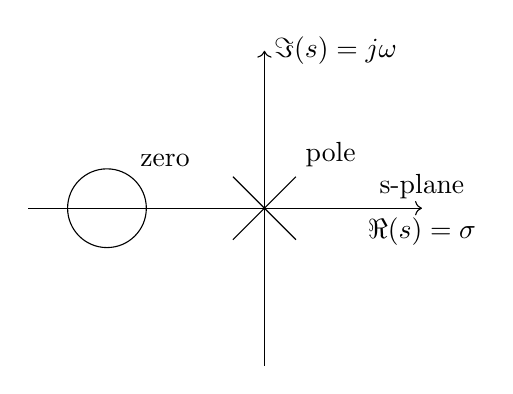
\begin{tikzpicture}
			\draw[->] (-3,0) -- (2,0) node[below]{$\Re(s)=\sigma$};
			\draw[->] (0,-2) -- (0,2) node[right]{$\Im(s)=j\omega$};
			\draw (-2,0) circle [radius=0.5];
			\draw(-1.7,0.4) node[ above right]{zero};
			\draw[-] (-0.4,0.4) -- (0.4,-0.4);
			\draw[-] (-0.4, - 0.4) -- (0.4,0.4) node[above right]{pole};
			\draw (2,0) node[above] {s-plane};
		\end{tikzpicture}
		\caption{Pole zero plot of a transfer function, with $k=1$}
	\end{figure}

\subsection{Poles and Responses}
	TF
	\begin{equation}
		G(s) = \frac{N(s)}{D(s)}
	\end{equation}

\subsubsection{Case of real poles}
	Suppose
	\begin{equation}
		G(s) = \frac{k N(s)}{(s+a)(s+b)(s+c)}
	\end{equation}
	Where $a, b, c\cdot$ are real and $k$ is a constant.

		The output when a step input (ie, $\frac{1}{s}$) is applied (i.e. the step response) is
	\begin{eqnarray}
		\frac{k N(s)}{s(s+a)(s+b)(s+c)} &=&  \frac{k_0}{s} + \frac{k_1}{s+a} +  \frac{k_2}{s+b} + \frac{k_3}{s+c} +\cdot \nonumber \\
		&=& \frac{k_0}{s} + \mbox{remainder terms}
	\end{eqnarray}
	where $k_n$ are constants.

	Note:
	\begin{itemize}
		\item Poles determine the form of response
		\item Zeros determine the relative components (due to input and poles) to the overall response through $k_n$
		\item $\frac{k_0}{s}$ is due to input and remainder term is due to poles
	\end{itemize}

	Inverse LT of remainder terms gives:
	\begin{equation}
		k_1e^{-at}+k_2e^{-bt}+k_3e^{-ct}+\cdot
		\label{eq:invltreal}
	\end{equation}
	Where $k_1, k_2, k_3 \cdot$ are affected by $N(s)$ and exponential terms depend on inputs. This is an exponential response.

\subsubsection{Case of complex poles}
	Suppose $D(s)$ also has complex poles at $s=-\alpha\pm j\beta$. Each pair of xomplexce poles gives rise to 
	\begin{equation}
		\frac{As+B}{(s+\alpha)^2+\beta^2}
	\end{equation}
	in the step response, where $A$ and $B$ are constants.

	Let  $B=A\alpha + C\beta$ and expand
	\begin{equation}
		=\frac{A(s+\alpha)}{(s+\alpha)^2+\beta^2}+\frac{C\beta}{(s+\alpha)^2+\beta^2}
	\end{equation}
	Inverse LT gives
	\begin{equation}
		Ae^{-\alpha t}\cos{\beta t}+Ce^{-\beta t}\sin{\beta t}= Re^{-\alpha t} \sin{(\beta t+\phi)}
		\label{eq:invltcomplex}
	\end{equation}
	which gives rise to an oscillatory response.

	\begin{figure}[H]
		\centering
		\begin{subfigure}[b]{0.3\textwidth}
			\centering
			\begin{tikzpicture}
				\draw[->] (-0.5,0) -- (4,0) node[below]{$t$};
				\draw[->] (0, -0.5)  -- (0,3) node[above]{Response};
				\draw[domain=0:4, samples=200] plot(\x, {exp(-\x*1.1)});
				\draw[-] (-0.1,1) node[left]{$1$} -- (0.1,1);
				\draw[-] (0,0) node[below left]{$0$};
			\end{tikzpicture}
			\caption{For $s=-a$}
		\end{subfigure}
		\begin{subfigure}[b]{0.3\textwidth}
			\centering
			\begin{tikzpicture}
				\draw[->] (-0.5,0) -- (4,0) node[below]{$t$};
				\draw[->] (0, -0.5) -- (0,3) node[above]{Response};
				\draw[domain=0:2.19722, samples=200] plot(\x, {exp(\x/2)});
				\draw[-] (-0.1,1) node[left]{$1$} -- (0.1,1);
				\draw[-] (0,0) node[below left]{$0$};
			\end{tikzpicture}
			\caption{For $s=a$}
		\end{subfigure}
		\caption{Time waveforms corresponding to a pole at $s=\pm a$ where $a$ is positive}
	\end{figure}

	From equation \ref{eq:invltreal}, a pole at $s=-a$ (or $s=a$) gives rise to $e^{-at}$ (or $e^{at}$) in the system response which is non oscillatory and decaying (or growing). The larger the value of $a$, the faster the rate of decay (or growth).


	\begin{figure}[H]
		\centering
		\begin{subfigure}[b]{0.3\textwidth}
			\centering
			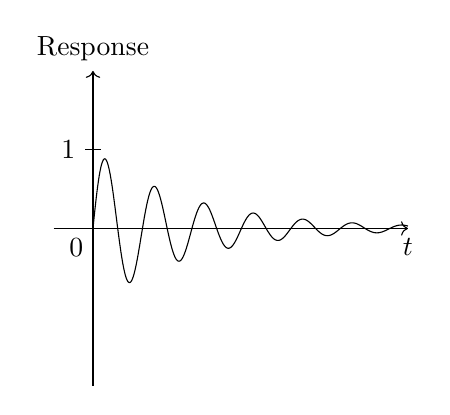
\begin{tikzpicture}
				\draw[->] (-0.5,0) -- (4,0) node[below]{$t$};
				\draw[->] (0, -2)  -- (0,2) node[above]{Response};
				\draw[domain=0:4, samples=400] plot(\x, {sin(\x*10 r) * exp(-\x*0.8)});
				\draw[-] (-0.1,1) node[left]{$1$} -- (0.1,1);
				\draw[-] (0,0) node[below left]{$0$};
			\end{tikzpicture}
			\caption{Negative real part}
		\end{subfigure}
		\begin{subfigure}[b]{0.3\textwidth}
			\centering
			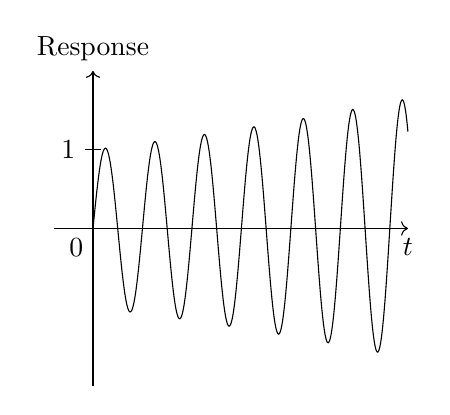
\begin{tikzpicture}
				\draw[->] (-0.5,0) -- (4,0) node[below]{$t$};
				\draw[->] (0, -2) -- (0,2) node[above]{Response};
				\draw[domain=0:4, samples=400] plot(\x, {sin(\x*10 r) * exp(\x/8)});
				\draw[-] (-0.1,1) node[left]{$1$} -- (0.1,1);
				\draw[-] (0,0) node[below left]{$0$};
			\end{tikzpicture}
			\caption{Positive real part}
		\end{subfigure}
		\caption{Time waveforms corresponding to a complex pole with a real part}
	\end{figure}

	From equation \ref{eq:invltcomplex}, a pair of complex poles at $s=-\alpha \pm j\beta$ (or $s=\alpha \pm j\beta$) gives rise to $e^{-\alpha t}\sin{(\beta t+\phi)}$ (or $e^{\alpha t}\sin{(\beta t+\phi)}$) that is sinusoidal and decays (or grows) exponentially. The larger the value of $\alpha$ the faster the rate of decay (or growth). $\beta$ determines the frequency of the oscillation.

	\begin{figure}[H]
		\centering
		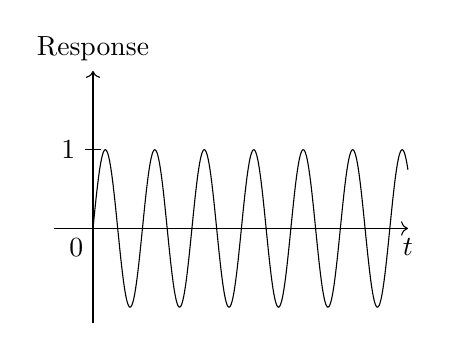
\begin{tikzpicture}
			\draw[->] (-0.5,0) -- (4,0) node[below]{$t$};
			\draw[->] (0, -1.2) -- (0,2) node[above]{Response};
			\draw[domain=0:4, samples=400] plot(\x, {sin(\x*10 r)});
			\draw[-] (-0.1,1) node[left]{$1$} -- (0.1,1);
			\draw[-] (0,0) node[below left]{$0$};
		\end{tikzpicture}
		\caption{Time waveform corresponding to a complex pole on the imaginary axis of the Laplace s-plane}
	\end{figure}
	From equation \ref{eq:invltcomplex}, if a pair of complex poles are on the imaginary axis (i.e. $\alpha=0$) then response is sinusoidal where $\beta$ determines the frequency of oscillation.

\section{}
\section{Z Transform (ZT)}
For a causal sequence $\left\{ x(n) \right\}$, ie $x(n)=0$ for $n<0$,
\begin{equation}
\left\{x(n)\right\} = \left\{x(0),x(1), x(2) \cdot x(n)\cdot\right\}
\end{equation}
its ZT is
\begin{equation}
X(z) = \sum^\infty_{n=0}x(n)z^-n
\end{equation}
Where z is a complex variable, and $z^{-n}$ denotes the position in time of $x(n)$.

\begin{example}
	\begin{eqnarray}
		\left\{x(n)\right\} &=& \left\{2, 4, 1, 0, 6 \cdots \right\} \nonumber \\
		X(z) &=&  2 z^0+4z^{-1} + z^{z-2}+0z^{-3}+6z^{-4}+\cdots
	\end{eqnarray}
\end{example}
Inverse ZT
\begin{eqnarray}
	X(z)= x(0)z^0+x(1)z^{-1}+x(2)z^{-2}+\cdots+x(n)z^{-n} + \cdots \nonumber \\
	\{x(n)\}&=&\{x(0), x(1), x(2), \cdots, x(n), \cdots \}
\end{eqnarray}
\begin{example}
	\begin{eqnarray}
		X(z) &=& \frac{z^{-2}-z^{-7}}{1-z{-1}} \\
		X(z) &=& (z^{-2}-z^{-7})(1+z^{-1}+z^{-2}+\cdots+z^{-n} + \cdots\nonumber \\
		&=& z^{-2}+z^{-3}+z^{-4}+z^{-5}+z^{-6} \nonumber \\
		\{x(n)\}&=&\{0,0,1,1,1,1,1\}
\end{eqnarray}
\end{example}

\subsection{Properties of ZT}
\begin{enumerate}
\item Linearity
${x_1(n)}\leftrightarrow X_1(z)$ and ${x_2(n)}\leftrightarrow X_2(z)$ then ${x_1(n)}+{x_2(n)}\leftrightarrow X_1(z)+X_2(z)$
\item
Time shifting
\begin{eqnarray}
{y(n)}&=&{x(n-m)}\nonumber \\
Y(z) &=& z^{-m}X(z)
\end{eqnarray}
ie, multiplying by $z^{-m}$ results in a delay of m sampling intervals.

\begin{example}
	\begin{eqnarray}
		\left\{x(n)\right\} &=& \{5,4,3,2,1\} \nonumber \\
		\{y(n)\} &=& \{-,5,4,3,2,1\} \nonumber \\
		Y(z) &=& 0z^0+5z^{-1}+4z^{-2}+3z^{-3}+2z^{_4}+z^{-5} \nonumber \\
		&=& z^{-1}(5+4z^{-1}+3z^{-2}+2z^{-3}+z^{-4}) \nonumber \\
		&=& z^{-1}(X(z))
\end{eqnarray}
$y(n)$ is $x(n)$ delayed by one.
\end{example}
\item Scaling
\begin{equation}
k\{x(n)\}=\leftrightarrow kX(z)
\end{equation}
\end{enumerate}

\subsection{ZT transfer function (ZT TF)}
For a linear system ZT TF\begin{equation}
 H(z) = \frac{C(z)}{R(z)}
\end{equation}
Where $\{c(n)\}$ is an output sequence and  $\{r(n)\}$  is an input sequence

\subsection{Pulse transfer function}
For $H(z)=\frac{C(z)}{R(z)}$ if $\{r(n)\} = \{1,0,0,\cdots\}$ (a unit impulse, ie, $R(z)=1$), then $C(z)=H(z)$ (pulse TF, which characterises the system).

$\{c(n)\}$ - Impulse response (IR) 
\begin{equation}
	\{c(n)\} = \{h(n)\} \leftrightarrow H(z)
\end{equation}
 ie pulse TF is ZT of IR.

\subsection{Linear shift Invariant (LSI) operations on sequences}
\begin{enumerate}

\item Multiplier (see Figure \ref{fig:multiplier})
	\begin{figure}[h]
		\centering
		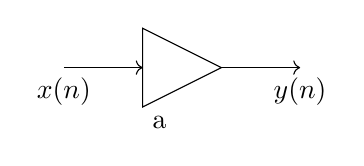
\begin{tikzpicture}
			\draw[->] (0,0) node[below]{$x(n)$} -- (1,0);
			\draw[-] (1,0) -- +(0,0.5)  -- +(1,0) -- +(0,-0.5) node [below right]{a}--+(0,0);
			\draw[->] (2,0) -- (3,0) node[below]{$y(n)$};
		\end{tikzpicture}
		\caption{A multiplier}
		\label{fig:multiplier}
	\end{figure}

\begin{equation}
	\{y(n)\} = \{ a x(0), ax(1), \cdots, ax(n), \cdots \}
\end{equation}

\item Adder (see Figure \ref{fig:adder})
	\begin{figure}[h]
		\centering
		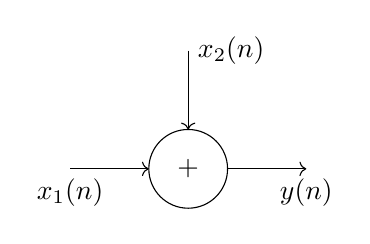
\begin{tikzpicture}
			\draw[->] (0,0) node[below]{$x_1(n)$} -- (1,0);
			\draw (1.5,0) node{$+$} circle(0.5);
			\draw[->] (1.5,1.5) node[right]{$x_2(n)$} -- (1.5,0.5);
			\draw[->] (2,0) -- (3,0) node[below]{$y(n)$};
		\end{tikzpicture}
		\caption{An adder}
		\label{fig:adder}
	\end{figure}

\begin{equation}
	\{y(n)\} = \{ x_1(0)+x_2(0),x_1(1)+x_2(1), \cdots\}
\end{equation}

\item Delay unit (see Figure \ref{fig:delay})
	\begin{figure}[h]
		\centering
		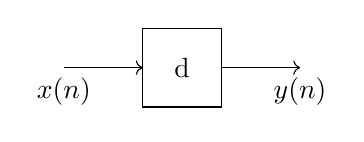
\begin{tikzpicture}
			\draw[->] (0,0) node[below]{$x(n)$} -- (1,0);
			\draw[-] (1,0) -- +(0,0.5)  -- +(1,0.5) -- +(1,-0.5)-- +(0,-0.5) --+(0,0);
			\draw (1.5,0) node {d};
			\draw[->] (2,0) -- (3,0) node[below]{$y(n)$};
		\end{tikzpicture}
		\caption{A delay unit}
		\label{fig:delay}
	\end{figure}

\begin{equation}
	\{y(n)\} = D\{x(n)\}=\{x(n-1)\}
\end{equation}
\begin{example}
	A moving averager (see Figure \ref{fig:averager})
	\begin{figure}[h]
		\centering
		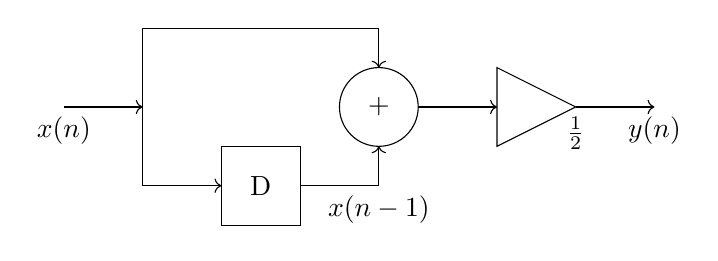
\begin{tikzpicture}
			\draw[->] (0,0) node[below]{$x(n)$} -- (1,0); % draw input node
			\draw[<->] (2,-1) -- (1,-1) -- (1,1) -- (4,1) -- (4,0.5); % Draw paths
			\draw (4,0) node{$+$} circle(0.5); % draw adder
			\draw[-] (2,-1) -- +(0,0.5)  -- +(1,0.5) -- +(1,-0.5)-- +(0,-0.5) --+(0,0); % draw delay unit
			\draw (2.5,-1) node {D}; % draw d in delay unit
			\draw[->] (3,-1)  -- (4,-1) node[below]{$x(n-1)$} -- (4,-0.5); % arrow to adder
			\draw[->] (4.5,0) -- +(1,0); % arrow to multiplier
			\draw[-] (5.5,0) -- +(0,0.5)  -- +(1,0) node [below]{$\frac{1}{2}$} -- +(0,-0.5) --+(0,0);
			\draw[->] (6.5,0) -- +(1,0) node[below]{$y(n)$}; % arrow to multiplier
		\end{tikzpicture}
		\caption{A moving averager}
		\label{fig:averager}
	\end{figure}
	
	\begin{eqnarray}
		y(n) &=& \frac{z(n)+x(n-1)}{2} \nonumber \\
		\left\{y(n)\right\} &=& \frac{\{z(n)\}+\{x(n-1)\}}{2} \nonumber \\
		Y(z) &=& \frac{X(z)+Z^{-1}X(Z)}{2} \nonumber \\
		H(z) &=& \frac{Y(z)}{X(z)} = \frac{1-z^{-1}}{2} = \frac {z+1}{2}
	\end{eqnarray}
\end{example}
\end{enumerate}
\end{document}